\documentclass[10pt]{article}
\usepackage[margin=0.8in]{geometry}
\usepackage{booktabs,graphicx,microtype,amsmath,array,enumitem,xcolor}
\usepackage[font=small,labelfont=bf,skip=3pt]{caption}
\usepackage[colorlinks=true,linkcolor=blue!50!black,citecolor=blue!50!black,urlcolor=blue!50!black]{hyperref}
\usepackage{listings}
\lstset{basicstyle=\ttfamily\scriptsize,breaklines=true,columns=fullflexible,frame=single,framerule=0.2pt}
\setlist{nosep,leftmargin=1.2em}
\setlength{\parskip}{3pt}\setlength{\parindent}{0pt}
\newcommand{\tb}[1]{\resizebox{\linewidth}{!}{#1}}
\newcommand{\code}[1]{\texttt{\small #1}}

\title{\vspace{-1.2cm}\textbf{2D Object Detection under Domain Shift:\\ A Reproducible Evaluation of YOLO11, RT-DETR, Faster R-CNN and FCOS\\ on COCO and KITTI}\\[2pt]
\large CMPE-249 Intelligent Autonomous Systems -- Homework: 2D Detection Survey and Evaluation (Track A)}
\author{Trevor ONeil}
\date{October 2026}

\begin{document}
\maketitle
\vspace{-0.8cm}
\begin{abstract}\small
I evaluate four COCO-pretrained detectors from four design families -- YOLO11s (anchor-free, task-aligned assignment, NMS), RT-DETR-L (query-based, Hungarian matching, NMS-free), Faster R-CNN R50-FPN (anchor-based two-stage) and FCOS R50-FPN (anchor-free one-stage) -- on the full COCO val2017 set (5000 images) and, \emph{without retraining}, on a 1000-image random subset of the KITTI 2D object detection training split. All numbers come from one harness (\code{evaluate.py}) running on an RTX~4050 Laptop GPU (6~GB). COCO numbers reproduce the published values within $\le$1.5 mAP, which validates the harness. Zero-shot on KITTI the 3-class mAP drops by 41\%, 39\%, 25\% and 22\% for YOLO11s, RT-DETR-L, Faster R-CNN and FCOS; the damage is concentrated on \emph{person} (AP 52--62 $\rightarrow$ 27--29) and \emph{truck}, while \emph{car} does not degrade at all. A large part of the gap for the two 640-pixel models is an \emph{input-resolution} effect of KITTI's 3.3:1 aspect ratio (YOLO11s gains +3.8 mAP at 1280 px), not semantic domain shift. I further analyse NMS vs.\ NMS-free inference (measuring duplicate boxes directly), the speed--accuracy trade-off (including a finding that batch-1 YOLO latency is kernel-launch-bound on this machine), and give a failure analysis by object size, occlusion and label confusion. All code, logs and raw results are in \code{detection\_hw/}.
\end{abstract}

%------------------------------------------------------------------
\section{Goals and Questions}
The task is to design, reproduce and critically analyse a meaningful detection experiment. I ask three questions: \textbf{(Q1)} how much does a COCO-pretrained detector degrade zero-shot on an autonomous-driving dataset, and which classes and scales suffer most? \textbf{(Q2)} Do the architectural differences between detector families (anchors vs.\ anchor-free vs.\ queries; NMS vs.\ set prediction) leave measurable fingerprints in the outputs? \textbf{(Q3)} What does the speed--accuracy trade-off look like on commodity laptop hardware? I deliberately report where my measurements \emph{disagree} with the textbook expectation (Sec.~\ref{sec:speed}).

%------------------------------------------------------------------
\section{Models and Datasets}
\subsection{Detector configurations}
Four configurations from four families were evaluated end-to-end (Table~\ref{tab:models}); YOLO11n/m were additionally run on KITTI only to trace a size frontier. Architectural facts in Table~\ref{tab:models} were read from the installed library source (paths relative to \code{site-packages/}) and model YAMLs, not from papers.

\begin{table}[h]\centering\footnotesize
\caption{Evaluated configurations. Source references verified in the installed packages (torchvision 0.29.1, ultralytics 8.4.193).}\label{tab:models}
\renewcommand{\arraystretch}{1.15}
\newcolumntype{R}[1]{>{\raggedright\arraybackslash}p{#1}}\begin{tabular}{@{}R{1.45cm}R{3.55cm}R{3.55cm}R{3.7cm}R{3.1cm}@{}}
\toprule
 & \textbf{YOLO11s} & \textbf{RT-DETR-L} & \textbf{Faster R-CNN} & \textbf{FCOS} \\
\midrule
Checkpoint & \code{yolo11s.pt} (9.5M) & \code{rtdetr-l.pt} (33.0M) & torchvision \code{fasterrcnn\_resnet50\_fpn} \code{COCO\_V1} (41.8M) & torchvision \code{fcos\_resnet50\_fpn} \code{COCO\_V1} (32.3M) \\
Backbone & C3k2 blocks + SPPF + C2PSA (\code{yolo11.yaml}) & HGNetv2 (\code{HGStem}/\code{HGBlock} in \code{rtdetr-l.yaml}) & ResNet-50 & ResNet-50 \\
Neck & PAN-FPN (top-down + bottom-up, \code{Concat}+C3k2), P3--P5 & Hybrid encoder: \code{AIFI} on S5 + \code{RepC3} FPN/PAN fusion & FPN P2--P6 & FPN P3--P7 (\code{LastLevelP6P7}, \code{fcos.py:768}) \\
Head / paradigm & Decoupled, anchor-free; DFL box distribution (\code{reg\_max=16}, \code{nn/modules/head.py:108}) & \code{RTDETRDecoder}, 300 queries, deformable attention (\code{head.py:1530}) & RPN (5 levels $\times$ 3 aspect ratios) + RoI box head, anchor-based, two-stage & Dense per-location class / box / centerness, anchor-free \\
Target assignment & Task-aligned (\code{utils/tal.py:14}, $\alpha{=}1,\beta{=}6$, top-10 in \code{loss.py:359}) & Hungarian (\code{models/utils/ops.py:15}), costs class:2 bbox:5 giou:2 (\code{models/utils/loss.py:68}) & IoU matcher: RPN 0.7/0.3, RoI 0.5/0.5 (\code{faster\_rcnn.py:184--197}) & Centre sampling (radius 1.5), per-level scale ranges, min-area tie-break (\code{fcos.py:440--483}) \\
Loss & BCE cls; CIoU + DFL box (\code{loss.py:142,148,465}) & set loss (cls + L1 + GIoU) with denoising queries & CE + smooth-L1 (\code{roi\_heads.py:12--45}, \code{rpn.py:325}) & focal + GIoU + centerness BCE (\code{fcos.py:91,97,117}) \\
Post-proc. & class-aware NMS, IoU 0.7 (\code{utils/nms.py:146}) & \textbf{none}: top-$k$ over flattened query$\times$class scores (\code{head.py:1727}) & NMS 0.7 on proposals (\code{rpn.py:289}), then class-wise NMS 0.5 (\code{roi\_heads.py:728}) & top-1000 candidates, class-wise NMS 0.6 (\code{fcos.py:545}) \\
Input pipeline & letterbox, long side 640 & \textbf{stretch} to 640$\times$640 (\code{rtdetr/predict.py}: \code{scale\_fill = True}) & resize short side 800 / long $\le$1333 & same as Faster R-CNN \\
\bottomrule
\end{tabular}
\end{table}

\subsection{Datasets and label mapping}
\textbf{COCO val2017}: all 5000 images, official annotations; reported both over 80 classes and over the 3-class subset {person, car, truck} used on KITTI so that the two datasets are comparable.\\
\textbf{KITTI}: the official 2D-detection \emph{training} split has 7481 images; I sampled 1000 uniformly at random (seed 0) and fetched only those PNGs from the 12.5~GB archive via HTTP range requests (\code{prepare\_data.py}). The subset contains 4261 car/van, 568 pedestrian/sitting-person, and 147 truck boxes. KITTI classes are mapped to COCO as follows:
\begin{itemize}
\item Car, Van $\rightarrow$ \emph{car}; Truck $\rightarrow$ \emph{truck}; Pedestrian, Person\_sitting $\rightarrow$ \emph{person}.
\item Cyclist $\rightarrow$ ignore region for person \emph{and} bicycle (COCO detectors predict rider and bike separately; KITTI has one box). Tram, Misc $\rightarrow$ ignore for car/truck. DontCare $\rightarrow$ ignore for all three classes. Ignore regions are COCO \code{iscrowd=1} boxes, so a detection inside them is neither TP nor FP under \code{pycocotools}.
\item All other COCO predictions (bus, train, bicycle, \dots) are discarded before scoring. No KITTI difficulty filtering is applied (all heights, all occlusion levels), so the numbers are \emph{not} comparable to the KITTI leaderboard.
\end{itemize}
Table~\ref{tab:stats} shows that the two datasets differ strongly in size and occlusion statistics, which matters for interpreting Q1.

\begin{table}[h]\centering\footnotesize
\caption{Ground-truth statistics (computed by \code{extra\_analysis.py}). Heights in pixels of the \emph{original} image.}\label{tab:stats}
\tb{\begin{tabular}{llrrrrr}
\toprule
Set & Class & \#GT & median box h (px) & \% small/$h{<}40$ & \% occluded & \% truncated \\
\midrule
COCO val & person & 10777 & 83 & 40 (area$<32^2$) & -- & -- \\
COCO val & car & 1918 & 26 & 62 (area$<32^2$) & -- & -- \\
COCO val & truck & 414 & 55 & 28 (area$<32^2$) & -- & -- \\
\midrule
KITTI subset & person & 568 & 89 & 12 & 43 & 5 \\
KITTI subset & car & 4261 & 47 & 40 & 55 & 12 \\
KITTI subset & truck & 147 & 60 & 33 & 46 & 13 \\
\bottomrule
\end{tabular}
}
\end{table}

%------------------------------------------------------------------
\section{Experimental Setup (Reproducibility)}
\textbf{Hardware/software.} Acer laptop, NVIDIA GeForce RTX 4050 Laptop GPU (6~GB, driver 546.18), Windows 11 (10.0.26200), Python 3.12.6, PyTorch 2.14.1+cu126, torchvision 0.29.1, Ultralytics 8.4.193, pycocotools; fp32 everywhere unless stated (default PyTorch precision settings). Measured raw fp32 matmul throughput is only 2.85~TFLOPS (the laptop GPU is power limited), so \emph{absolute} latencies are higher than on desktop GPUs; only relative comparisons are meaningful.\\
\textbf{Accuracy protocol.} Confidence threshold 0.001, max 100 detections/image for all models, NMS IoU = each library's default (YOLO 0.7, Faster R-CNN 0.5, FCOS 0.6, RT-DETR n/a). YOLO/RT-DETR run at \code{imgsz=640}; torchvision models at their default min\_size 800 / max\_size 1333. Metrics are COCO-style (\code{COCOeval}, bbox): mAP@[.5:.95], AP$_{50}$, AP$_{75}$, AP$_{S/M/L}$, AR$_{100}$, per-class AP from the precision tensor. \textbf{Latency protocol} (\code{bench\_latency.py}): batch 1, conf 0.25, CUDA-synchronised wall-clock for resize + forward + decode + NMS (JPEG decode excluded); 100 images per dataset, each model (re)loaded and warmed up on 40 images, 3 interleaved rounds, median of round-medians. Peak memory is \code{max\_memory\_allocated} (weights + activations, excluding the CUDA context). Throughout, ``failure analysis'' uses score $\ge$0.3 and IoU $\ge$0.5.\\
\textbf{Commands.} Full command log in Appendix~\ref{app:cmd} (\code{run\_all.ps1}); per-run logs in \code{results/logs/}, metrics JSON in \code{results/*.json}.

%------------------------------------------------------------------
\section{Quantitative Results}
\begin{table}[h]\centering\footnotesize
\caption{Main accuracy results (\%). ``3 cls'' = person, car, truck. COCO 80-class numbers: YOLO11s 45.5 (official 47.0 at 300 dets), RT-DETR-L 52.6 (53.0), Faster R-CNN 37.2 (37.0), FCOS 39.2 (39.2).}\label{tab:main}
\tb{\begin{tabular}{llrrrrrrr}
\toprule
Model & Eval set & mAP & AP$_{50}$ & AP$_{75}$ & AP$_S$ & AP$_M$ & AP$_L$ & AR$_{100}$ \\
\midrule
YOLO11s & COCO val, 80 cls & 45.5 & 62.0 & 49.2 & 27.6 & 50.1 & 62.5 & 60.2 \\
 & COCO val, 3 cls & 46.3 & 65.7 & 49.9 & 27.7 & 55.6 & 69.7 & 60.6 \\
 & KITTI, 3 cls & 27.4 & 50.2 & 27.4 & 16.6 & 25.6 & 39.8 & 43.4 \\
\midrule
RT-DETR-L & COCO val, 80 cls & 52.6 & 70.9 & 57.0 & 33.9 & 57.3 & 70.7 & 69.0 \\
 & COCO val, 3 cls & 52.4 & 74.5 & 56.2 & 33.9 & 61.1 & 75.4 & 69.4 \\
 & KITTI, 3 cls & 32.0 & 55.6 & 31.7 & 22.1 & 31.6 & 44.0 & 56.1 \\
\midrule
Faster R-CNN & COCO val, 80 cls & 37.2 & 59.0 & 39.9 & 21.3 & 40.5 & 48.4 & 53.0 \\
 & COCO val, 3 cls & 41.8 & 68.8 & 43.8 & 28.6 & 49.0 & 56.2 & 58.4 \\
 & KITTI, 3 cls & 31.4 & 57.7 & 31.1 & 35.1 & 29.9 & 40.6 & 52.5 \\
\midrule
FCOS & COCO val, 80 cls & 39.2 & 58.3 & 42.0 & 22.2 & 42.4 & 51.3 & 57.1 \\
 & COCO val, 3 cls & 43.2 & 66.4 & 46.2 & 28.1 & 49.9 & 61.5 & 61.3 \\
 & KITTI, 3 cls & 33.6 & 59.0 & 35.9 & 28.1 & 31.7 & 43.3 & 52.5 \\
\bottomrule
\end{tabular}
}
\end{table}

\begin{table}[h]\centering\footnotesize
\caption{Per-class AP (\%) on COCO val vs.\ the KITTI subset, same three classes.}\label{tab:perclass}
\tb{\begin{tabular}{llrrrrrr}
\toprule
 & & \multicolumn{3}{c}{AP@[.5:.95]} & \multicolumn{3}{c}{AP$_{50}$} \\
\cmidrule(lr){3-5}\cmidrule(lr){6-8}
Model & Set & person & car & truck & person & car & truck \\
\midrule
YOLO11s & COCO & 58.6 & 44.8 & 35.5 & 81.4 & 66.2 & 49.4 \\
 & KITTI & 27.4 & 45.0 & 9.6 & 58.1 & 78.4 & 14.1 \\
\midrule
RT-DETR-L & COCO & 61.5 & 49.9 & 45.8 & 85.9 & 73.4 & 64.1 \\
 & KITTI & 28.3 & 49.9 & 17.7 & 59.7 & 82.6 & 24.6 \\
\midrule
Faster R-CNN & COCO & 51.8 & 41.1 & 32.5 & 82.1 & 68.2 & 56.2 \\
 & KITTI & 29.2 & 44.8 & 20.2 & 61.7 & 79.9 & 31.4 \\
\midrule
FCOS & COCO & 53.3 & 42.2 & 34.2 & 80.6 & 65.2 & 53.4 \\
 & KITTI & 28.4 & 47.6 & 24.8 & 58.3 & 82.4 & 36.3 \\
\bottomrule
\end{tabular}
}
\end{table}

\begin{table}[h]\centering\footnotesize
\caption{Latency, memory and size (controlled benchmark, batch 1, conf 0.25; median of 3 interleaved rounds; round-to-round spread is $\le$12\% for torchvision/RT-DETR and up to $\sim$35\% for the small YOLO models).}\label{tab:latency}
\tb{\begin{tabular}{lrrrrrrrr}
\toprule
Model & Params (M) & \multicolumn{2}{c}{fp32 ms (KITTI / COCO)} & \multicolumn{2}{c}{fp16 ms (KITTI / COCO)} & \multicolumn{2}{c}{Peak mem. MB (fp32, KITTI / COCO)} & FPS$_{\rm fp32}$ COCO \\
\midrule
YOLO11n & 2.6 & 38 & 39 & 41 & 38 & 18 & 34 & 25.5 \\
YOLO11s & 9.5 & 30 & 35 & 39 & 35 & 51 & 79 & 28.2 \\
YOLO11m & 20.1 & 44 & 49 & 51 & 48 & 106 & 158 & 20.4 \\
RT-DETR-L & 33.0 & 113 & 107 & 102 & 91 & 213 & 213 & 9.3 \\
Faster R-CNN & 41.8 & 149 & 203 & 125 & 157 & 424 & 657 & 4.9 \\
FCOS & 32.3 & 135 & 193 & 123 & 151 & 283 & 422 & 5.2 \\
\bottomrule
\end{tabular}
}
\end{table}

%------------------------------------------------------------------
\section{Technical Analysis}
\subsection{Cross-dataset generalisation (Q1)}
\textbf{Overall.} Restricted to the same three classes, zero-shot KITTI mAP is 27.4 / 32.0 / 31.4 / 33.6 (YOLO11s / RT-DETR-L / Faster R-CNN / FCOS) versus 46.3 / 52.4 / 41.8 / 43.2 on COCO: relative drops of 41\%, 39\%, 25\% and 22\% (Table~\ref{tab:main}). The \emph{ranking flips}: RT-DETR-L is $+10.6$ mAP over Faster R-CNN on COCO but only $+0.6$ on KITTI, and FCOS, the weakest-but-one on COCO, is best on KITTI.

\textbf{Which classes.} Fig.~\ref{fig:perclass}/Table~\ref{tab:perclass}: \emph{person} AP falls from 51.8--61.5 to 27.4--29.2 for \emph{every} model (nearly identical KITTI values across families suggests a data-side cause), and \emph{truck} falls from 32.5--45.8 to 9.6--24.8. \emph{Car} AP is unchanged or higher (44.8$\rightarrow$45.0, 49.9$\rightarrow$49.9, 41.1$\rightarrow$44.8, 42.2$\rightarrow$47.6). The car result is \emph{not} evidence of robustness: KITTI cars are much larger than COCO cars (median height 47 px vs.\ 26 px; 62\% of COCO cars are ``small'' by area), so the scale distribution, not the domain, drives it.

\textbf{Which failures: localisation more than recognition.} For person, AP$_{50}$ drops moderately (YOLO11s 81.4$\rightarrow$58.1, RT-DETR 85.9$\rightarrow$59.7) but AP[.5:.95] drops 2.1$\times$; the AP/AP$_{50}$ ratio goes from 0.72 to 0.47 for these two models. So many KITTI pedestrians are \emph{found} but boxed with a different convention (KITTI boxes are tight on the visible body of thin objects, where a 3--4 px error already costs IoU; 43\% of pedestrians are occluded, Table~\ref{tab:stats}). For car, AP$_{50}$ rises sharply (66.2$\rightarrow$78.4 for YOLO11s) while AP does not, i.e.\ the AP/AP$_{50}$ ratio also falls (0.68$\rightarrow$0.57).

\textbf{Which scales.} AP$_S$ is the weakest bucket on both datasets (Table~\ref{tab:main}), but the \emph{pattern differs by model on KITTI}: Faster R-CNN has the best AP$_S$ (35.1), YOLO11s the worst (16.6) -- see the resolution confound below.

\textbf{Resolution is confounded with domain.} KITTI frames are 1242$\times$375 (3.3:1). YOLO letterboxes them to $\approx$640$\times$224 (scale 0.52$\times$), whereas the torchvision models see $\approx$1333$\times$403 (1.07$\times$). RT-DETR stretches the frame to a 640$\times$640 square (anisotropic: 0.52$\times$ horizontally, 1.7$\times$ vertically; \code{scale\_fill=True}). Raising the input to 1280 px (Table~\ref{tab:abl}) gives YOLO11s +3.8 mAP / +2.5 AP$_S$ and RT-DETR-L +2.8 mAP / +9.2 AP$_S$, putting RT-DETR-L at 1280 (34.8) above every default-resolution model. A plausible explanation of RT-DETR's comparatively high AP$_S$ at 640 (22.1 vs.\ 16.6 for YOLO11s) is that the stretch gives small, upright objects (pedestrians, distant cars) 1.7$\times$ more vertical pixels; I did not isolate this with a letterboxed RT-DETR run, so it remains a hypothesis. The practical conclusion: roughly 3--4 of the 19--20 mAP points lost by the 640 models are a pre-processing artefact that a deployment would simply fix.

\begin{figure}[t]\centering
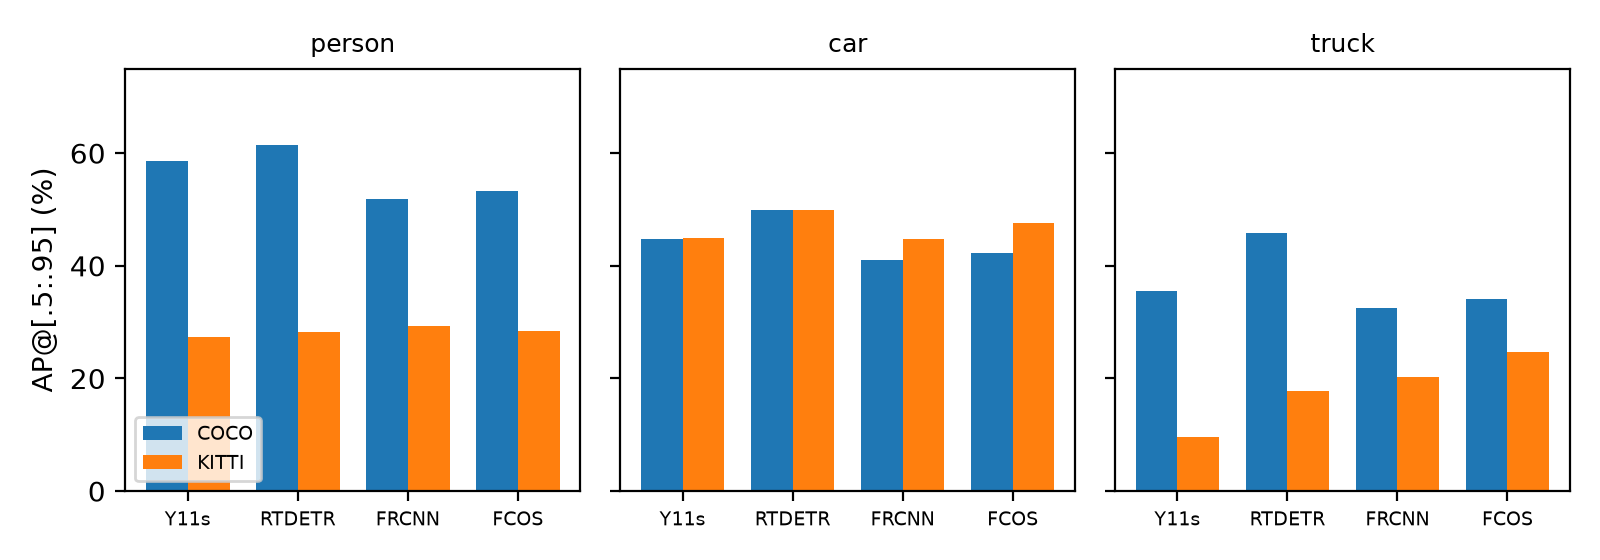
\includegraphics[width=0.78\linewidth]{fig_per_class.png}
\caption{Per-class AP@[.5:.95] on COCO val and KITTI subset (same 3 classes).}\label{fig:perclass}
\end{figure}

\begin{table}[t]\centering\footnotesize
\caption{KITTI ablations: NMS threshold, input resolution, model size (3-class AP, \%).}\label{tab:abl}
\tb{\begin{tabular}{lrrrrrr}
\toprule
Configuration (KITTI, 3 cls) & mAP & AP$_{50}$ & AP$_S$ & AP$_M$ & AP$_L$ & AR$_{100}$ \\
\midrule
YOLO11s, 640, NMS IoU 0.7 (default) & 27.4 & 50.2 & 16.6 & 25.6 & 39.8 & 43.4 \\
YOLO11s, 640, NMS IoU 0.3 & 26.4 & 48.1 & 16.5 & 24.2 & 38.6 & 40.2 \\
YOLO11s, 640, NMS IoU 0.5 & 26.8 & 49.3 & 16.6 & 24.8 & 39.2 & 41.5 \\
YOLO11s, 640, NMS IoU 0.9 & 26.9 & 48.0 & 15.6 & 24.8 & 40.3 & 45.3 \\
YOLO11s, 1280 & 31.2 & 55.6 & 19.1 & 31.7 & 40.4 & 48.2 \\
YOLO11n, 640 & 24.9 & 47.0 & 10.7 & 23.4 & 39.2 & 42.6 \\
YOLO11m, 640 & 30.4 & 54.5 & 22.4 & 28.6 & 43.0 & 48.2 \\
RT-DETR-L, 640 (no NMS) & 32.0 & 55.6 & 22.1 & 31.6 & 44.0 & 56.1 \\
RT-DETR-L, 1280 (no NMS) & 34.8 & 56.6 & 31.3 & 34.7 & 45.4 & 59.2 \\
Faster R-CNN, short side 800 (default) & 31.4 & 57.7 & 35.1 & 29.9 & 40.6 & 52.5 \\
FCOS, short side 800 (default) & 33.6 & 59.0 & 28.1 & 31.7 & 43.3 & 52.5 \\
\bottomrule
\end{tabular}
}
\end{table}

\subsection{Architecture comparison: NMS-based vs.\ NMS-free inference (Q2)}\label{sec:nms}
\textbf{Source-level difference.} YOLO11's \code{DetectionPredictor} (\code{models/yolo/detect/predict.py:55}) calls \code{non\_max\_suppression}, which offsets boxes by class index (\code{utils/nms.py:146}) so suppression is per class. Dense heads (YOLO, FCOS) emit many overlapping positives for one object because assignment is one-to-many: TAL gives each GT up to 10 anchors, FCOS every location inside the centre region. The NMS threshold is therefore a recall/precision hyper-parameter. RT-DETR instead trains with one-to-one Hungarian assignment (cost weights class 2 / bbox 5 / GIoU 2) so each GT is supervised on exactly one query; duplicates are penalised during training, and \code{RTDETRDecoder.postprocess} (\code{head.py:1710--1731}) just takes the top-$k$ of the flattened $300\times nc$ score matrix.

\textbf{Evidence 1: NMS threshold is a real knob.} Sweeping the NMS IoU of YOLO11s on KITTI (Table~\ref{tab:abl}): AR$_{100}$ 40.2 / 41.5 / 43.4 / 45.3 for IoU 0.3 / 0.5 / 0.7 / 0.9 and mAP 26.4 / 26.8 / 27.4 / 26.9. Aggressive NMS removes occluded neighbours in dense traffic (55\% of KITTI cars are occluded); too permissive NMS adds duplicates that cost precision. The best mAP is in the middle; a set-based detector has no such knob.

\textbf{Evidence 2: duplicates are measured directly.} At score $\ge$0.3 I counted same-class detections that overlap (IoU $\ge$0.5) a GT already claimed by a higher-scoring detection (Table~\ref{tab:dups}). RT-DETR's same-class duplicate rate (1.4\%) is \emph{lower} than YOLO11s's NMS-filtered 2.0\% and similar to Faster R-CNN's (1.5\%, which has two NMS stages), confirming that one-to-one training does suppress duplicates without NMS. But there is a new failure mode: RT-DETR yields \textbf{497} near-identical (IoU $\ge$0.9) \emph{cross-class} pairs versus 42 for YOLO11s. Because top-$k$ runs over query$\times$class scores, one query can be emitted twice with two labels (plausibly car vs.\ truck, the dominant label confusion in Sec.~\ref{sec:fail}) and nothing de-duplicates across classes. FCOS has the most duplicates (3.1\% same-class, 2422 cross-class pairs) because its sigmoid scores are poorly calibrated for this domain (16.9k detections above 0.3 vs.\ 5.2k for YOLO11s) and its NMS is class-wise.

\textbf{Evidence 3: assignment shows up in score calibration.} On KITTI, YOLO11s (task-aligned assignment, which trains the classification score towards IoU) is the most ``confident-precise'' model (consistent with, though not proof of, this mechanism): only 599 car FPs among 4397 detections $\ge$0.3 vs.\ 4281 among 10951 for FCOS. This is why a fixed 0.3 threshold gives YOLO the lowest recall (73.0\%) and FCOS the highest (86.5\%): the models are operated at very different points of their PR curves, and AP (threshold-free) is the fairer comparison.

\begin{table}[t]\centering\footnotesize
\caption{Duplicate and false-positive statistics on KITTI at score $\ge$0.3 (only person/car/truck detections; FP = no same-class GT with IoU $\ge$0.5 and not inside an ignore region).}\label{tab:dups}
\tb{\begin{tabular}{lrrrrr}
\toprule
Model & dets$\geq$0.3 & TP & same-class dup. (\%) & cross-class dup. pairs & FP person / car / truck \\
\midrule
YOLO11s & 5232 & 3513 & 2.0 & 42 & 130 / 599 / 145 \\
RT-DETR-L & 8747 & 3991 & 1.4 & 497 & 350 / 1448 / 656 \\
Faster R-CNN & 11969 & 4046 & 1.5 & 97 & 1046 / 2910 / 440 \\
FCOS & 16924 & 4219 & 3.1 & 2422 & 1998 / 4281 / 2137 \\
\bottomrule
\end{tabular}
}
\end{table}

\subsection{Speed--accuracy trade-off (Q3)}\label{sec:speed}
\begin{figure}[t]\centering
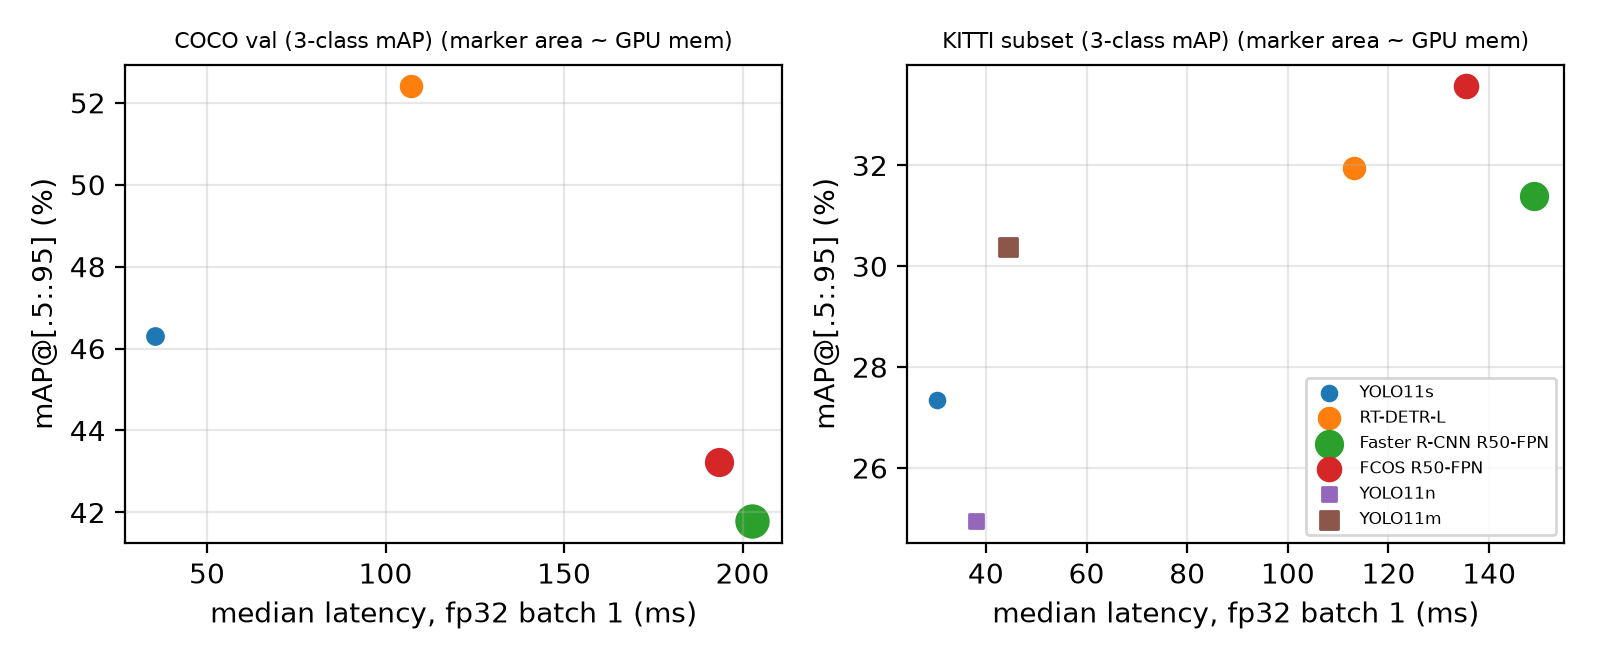
\includegraphics[width=0.95\linewidth]{fig_speed_acc.png}
\caption{3-class mAP vs.\ median batch-1 fp32 latency (Table~\ref{tab:latency}); marker area grows with peak GPU memory.}\label{fig:speed}
\end{figure}
\textbf{Pareto picture.} On COCO, RT-DETR-L (52.4 mAP, 107 ms) dominates both torchvision models (41.8 mAP @ 203 ms for Faster R-CNN, 43.2 @ 193 ms for FCOS): $\sim$2$\times$ faster, +9--11 mAP, and 2--3$\times$ less peak memory (213 vs.\ 657/422 MB). YOLO11s is the fastest (35 ms) at 6.1 mAP below RT-DETR-L. On KITTI the torchvision models become relatively cheaper (smaller image: 149/135 ms) and FCOS is on the Pareto front for accuracy (33.6), but YOLO11m (30.4 mAP @ 44 ms) nearly matches Faster R-CNN (31.4 @ 149 ms), and RT-DETR-L at 1280 px is the most accurate configuration overall (34.8 mAP, $\sim$255 ms in a single uncontrolled pass).

\textbf{A surprise: small YOLOs are not compute-bound at batch 1.} YOLO11n (6.5 GFLOPs), 11s (21.6) and 11m (68.1) take 38, 30 and 44 ms -- almost size-independent, and the 11s run is faster than 11n. The Ultralytics per-stage timers show 25--35 ms in the \emph{network} stage for all three (Table~\ref{tab:breakdown}), yet the same fused network at batch 16 costs only 4.3 / 7.4 / 18.0 ms \emph{per image}. At batch 1 these models are therefore limited by CPU-side kernel launching/driver overhead (Windows WDDM), not by FLOPs, which also explains why fp16 does not help them (YOLO11s 35$\rightarrow$35 ms, YOLO11n 39$\rightarrow$38) but does help the heavier models (Faster R-CNN 203$\rightarrow$157 ms, FCOS 193$\rightarrow$151, RT-DETR-L 107$\rightarrow$91). Consequence: FLOPs/parameter counts predict neither ranking nor speed at batch 1 here; a single-stream real-time deployment would need CUDA graphs/TensorRT, whereas offline evaluation benefits from batching ($\sim$5$\times$ for YOLO11n). I flag this because first-pass single-run timings in my own harness (e.g.\ 57 ms for YOLO11s on the first KITTI run vs.\ 30 ms in the controlled benchmark) were misleading until I interleaved models and warmed the GPU up.

\begin{table}[t]\centering\footnotesize
\caption{YOLO/RT-DETR latency breakdown on KITTI (ms, median of 100 images; ``pre/network/post'' from Ultralytics' timers) and raw fused-network time per image at batch 1 vs.\ 16 ($640\times640$ input).}\label{tab:breakdown}
\tb{\begin{tabular}{lrrrrrr}
\toprule
Model (KITTI, fp32) & pre & network & post & wall & net.\ @bs1 & net.\ per img @bs16 \\
\midrule
YOLO11n & 2.6 & 24.9 & 3.8 & 31.3 & 21.2 & 4.3 \\
YOLO11s & 2.2 & 30.0 & 4.2 & 37.1 & 31.9 & 7.4 \\
YOLO11m & 1.8 & 34.7 & 3.9 & 41.4 & 33.6 & 18.0 \\
RT-DETR-L & 4.8 & 101.4 & 2.0 & 109.5 & 93.0 & 29.6 \\
\bottomrule
\end{tabular}
}
\end{table}

%------------------------------------------------------------------
\section{Failure Analysis on KITTI}\label{sec:fail}
\begin{figure}[t]\centering
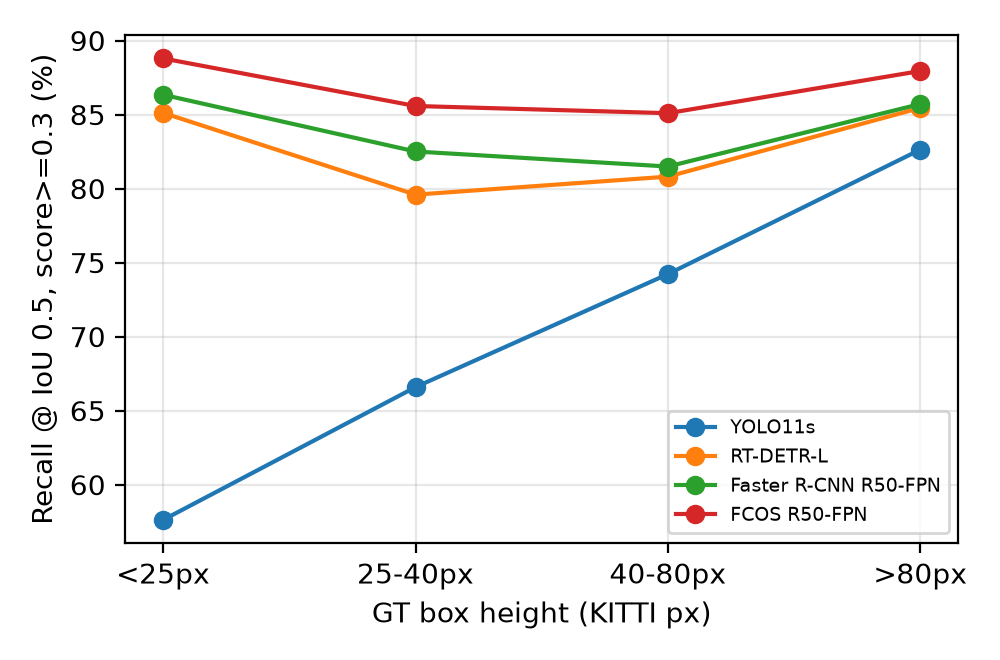
\includegraphics[width=0.48\linewidth]{fig_recall_height.png}
\caption{Recall@IoU 0.5 (score $\ge$0.3) vs.\ GT box height.}\label{fig:recallh}
\end{figure}
\begin{table}[t]\centering\footnotesize
\caption{Recall (\%) at score $\ge$0.3, IoU $\ge$0.5, by GT height (px) and class. $n$: 571 / 1269 / 1610 / 1526 objects per height bin; 568 / 4261 / 147 per class.}\label{tab:recall}
\tb{\begin{tabular}{lrrrrrrrr}
\toprule
 & \multicolumn{4}{c}{by GT box height} & \multicolumn{3}{c}{by class} & \\
\cmidrule(lr){2-5}\cmidrule(lr){6-8}
Model & $<$25 & 25--40 & 40--80 & $>$80 & person & car & truck & all \\
\midrule
YOLO11s & 57.6 & 66.6 & 74.2 & 82.6 & 59.2 & 76.3 & 28.6 & 73.0 \\
RT-DETR-L & 85.1 & 79.6 & 80.8 & 85.5 & 65.8 & 85.3 & 61.9 & 82.4 \\
Faster R-CNN & 86.3 & 82.5 & 81.5 & 85.7 & 70.2 & 85.8 & 70.7 & 83.6 \\
FCOS & 88.8 & 85.6 & 85.1 & 87.9 & 72.5 & 88.6 & 80.3 & 86.5 \\
\bottomrule
\end{tabular}
}
\end{table}
\begin{table}[t]\centering\footnotesize
\caption{Why a GT object is missed at score $\ge$0.3 (disjoint categories; ``low score'' = a correct-class box with IoU $\ge$0.5 exists but scores $<$0.3).}\label{tab:causes}
\tb{\begin{tabular}{lrrrrr}
\toprule
Model & low score & wrong class & poor loc. & nothing near & total missed \\
\midrule
YOLO11s & 669 & 125 & 319 & 233 & 1346 \\
RT-DETR-L & 367 & 11 & 382 & 115 & 875 \\
Faster R-CNN & 406 & 18 & 285 & 107 & 816 \\
FCOS & 228 & 18 & 337 & 88 & 671 \\
\bottomrule
\end{tabular}
}
\end{table}

\textbf{Small objects (Table~\ref{tab:recall}, Fig.~\ref{fig:recallh}).} YOLO11s at 640 px loses 25 recall points between $>$80 px (82.6\%) and $<$25 px (57.6\%) objects; the 800-px torchvision models and RT-DETR (vertically up-scaled) are almost flat (RT-DETR 85.1 / 79.6 / 80.8 / 85.5, FCOS 88.8 / 85.6 / 85.1 / 87.9 across the four height bins). This is the resolution effect of Sec.~5.1 seen at object level.

\textbf{Occlusion.} Recall on fully visible objects is 87--96\% but on ``largely occluded'' objects (KITTI level 2, 1049 boxes) it is only 46.6 / 58.0 / 59.9 / 64.8\% (YOLO11s / RT-DETR / Faster R-CNN / FCOS). By count, level-2 objects are the largest source of misses for every model (e.g.\ $\approx$560 of YOLO11s's misses at level 2 vs.\ $\approx$390 at level 1 and $\approx$300 at level 0, from recall $\times$ $n$): heavily occluded objects are low-confidence (``low score'' is the biggest category in Table~\ref{tab:causes} for YOLO11s: 669 of 1346 misses) or poorly localised (285--382 per model).

\textbf{Class confusion is mostly a taxonomy problem.} The ``wrong class'' misses are dominated by car$\rightarrow$truck (96 / 88 / 84 / 28 for YOLO11s / RT-DETR / Faster R-CNN / FCOS), car$\rightarrow$bus, truck$\rightarrow$train (27 for YOLO11s: long KITTI trucks and trailers) and truck$\rightarrow$bus. For \emph{truck} \emph{false positives} I traced where truck-labelled detections ($\ge$0.3) that do not match a KITTI Truck land (\code{taxonomy\_check.py}): for YOLO11s 112 of 177 sit on KITTI \emph{Vans} and 29 on Misc; for Faster R-CNN 185 of 546 on Vans and 123 on Cars; for FCOS 1232 of 2557 on ordinary Cars. KITTI's Van (mapped to car) is exactly the COCO ``truck/van'' boundary, so a large part of the low truck AP (9.6--24.8) is a label-definition mismatch plus only 147 truck instances (high variance), not a visual failure. Different Van policy (e.g.\ ignoring Vans for the truck class) would raise truck AP; I did not test it.

\textbf{Operating-point-dependent behaviour.} At 0.3, FCOS has the highest recall (86.5\%) but 8.4k person/car/truck FPs per 1000 images vs.\ 0.9k for YOLO11s (Table~\ref{tab:dups}); RT-DETR's extra truck FPs (656 vs.\ 145) are consistent with the cross-class duplicate mechanism of Sec.~\ref{sec:nms} (its non-matching truck boxes sit mostly on KITTI Cars and Vans, 297 and 257 of 771), though I did not trace individual duplicates.

%------------------------------------------------------------------
\section{Threats to Validity}
(1) KITTI is a 1000-image random subset of the training split; AP differences below $\sim$1 mAP between models (e.g.\ RT-DETR vs.\ Faster R-CNN) should not be over-interpreted, and truck AP rests on 147 instances. I did not compute confidence intervals. (2) Taxonomy choices (Van$\rightarrow$car, Cyclist/Tram/Misc as ignore) affect per-class numbers; the same protocol is applied to all models, so comparisons are fair, but absolute values are not KITTI-benchmark values. (3) Each model uses its \emph{native} pre-processing, so ``model'' and ``input resolution/aspect handling'' are confounded in the main table; the 1280 ablation and Sec.~5.1 partially disentangle it. (4) 100 detections/image for all models is slightly below Ultralytics' default of 300 (explaining part of the 1.5-point YOLO11s gap to the official 47.0). (5) Latencies come from a power-limited laptop GPU on Windows and are launch-bound for small models; they should not be extrapolated to other platforms. (6) No fine-tuning was performed; adapting to KITTI would be the obvious next experiment.

%------------------------------------------------------------------
\section{Conclusions}
\begin{enumerate}
\item The COCO$\rightarrow$KITTI gap is real but \emph{heterogeneous}: person and truck degrade strongly across \emph{all} families, car does not (a scale-distribution effect), and AP/AP$_{50}$ ratios show that box-convention and occlusion (localisation) hurt more than recognition.
\item Part of the apparent domain shift for 640-px models is a pre-processing artefact of KITTI's aspect ratio: 1280 px recovers +3--4 mAP for YOLO11s and RT-DETR-L (+9 AP$_S$ for the latter), and RT-DETR-L@1280 becomes the most accurate model overall (34.8 mAP).
\item NMS-free set prediction works as designed -- RT-DETR has fewer same-class duplicates (1.4\%) than NMS-filtered YOLO11s (2.0\%) -- but its flattened query$\times$class top-$k$ introduces cross-class duplicates (497 vs.\ 42) that class-aware NMS does not create. Dense one-to-many heads (YOLO/FCOS) need a tuned NMS threshold (AR$_{100}$ varies 40.2--45.3 across IoU 0.3--0.9).
\item On this machine RT-DETR-L gives the best COCO accuracy/latency trade-off among the large models (52.4 mAP at 107 ms vs.\ 41.8--43.2 at $\sim$200 ms), and small YOLOs are launch-bound at batch 1, so parameter or FLOP counts are poor predictors of latency; measurement protocol (warm-up, interleaving) changed my YOLO11s latency by almost 2$\times$.
\end{enumerate}

%------------------------------------------------------------------
\begin{thebibliography}{99}\footnotesize
\bibitem{fr} S.~Ren, K.~He, R.~Girshick, J.~Sun. Faster R-CNN: Towards Real-Time Object Detection with Region Proposal Networks. NeurIPS 2015 (arXiv:1506.01497).
\bibitem{fcos} Z.~Tian, C.~Shen, H.~Chen, T.~He. FCOS: Fully Convolutional One-Stage Object Detection. ICCV 2019 (arXiv:1904.01355).
\bibitem{detr} N.~Carion et al. End-to-End Object Detection with Transformers. ECCV 2020 (arXiv:2005.12872).
\bibitem{rtdetr} Y.~Zhao, W.~Lv, S.~Xu, et al. DETRs Beat YOLOs on Real-time Object Detection. CVPR 2024 (arXiv:2304.08069).
\bibitem{yolo11} R.~Khanam, M.~Hussain. YOLOv11: An Overview of the Key Architectural Enhancements. arXiv:2410.17725, 2024.
\bibitem{tood} C.~Feng et al. TOOD: Task-aligned One-stage Object Detection. ICCV 2021 (arXiv:2108.07755).
\bibitem{gfl} X.~Li et al. Generalized Focal Loss: Learning Qualified and Distributed Bounding Boxes. NeurIPS 2020 (arXiv:2006.04388).
\bibitem{focal} T.-Y.~Lin et al. Focal Loss for Dense Object Detection. ICCV 2017 (arXiv:1708.02002).
\bibitem{ciou} Z.~Zheng et al. Distance-IoU Loss: Faster and Better Learning for Bounding Box Regression (DIoU/CIoU). AAAI 2020 (arXiv:1911.08287).
\bibitem{coco} T.-Y.~Lin et al. Microsoft COCO: Common Objects in Context. ECCV 2014 (arXiv:1405.0312).
\bibitem{kitti} A.~Geiger, P.~Lenz, R.~Urtasun. Are we ready for Autonomous Driving? The KITTI Vision Benchmark Suite. CVPR 2012.
\bibitem{tv} PyTorch/TorchVision: \code{torchvision.models.detection} source and documentation, \url{https://github.com/pytorch/vision} (v0.29.1 inspected).
\bibitem{ul} Ultralytics: YOLO11 / RT-DETR implementation and documentation, \url{https://github.com/ultralytics/ultralytics} (v8.4.193 inspected).
\bibitem{pycoco} COCO API (\code{pycocotools}) and evaluation protocol, \url{https://cocodataset.org/\#detection-eval}.
\end{thebibliography}

%------------------------------------------------------------------
\appendix
\section{Command log and artefacts}\label{app:cmd}
\begin{lstlisting}
cd detection_hw
python -m venv .venv
.venv\Scripts\python -m pip install torch torchvision --index-url https://download.pytorch.org/whl/cu126
.venv\Scripts\python -m pip install ultralytics pycocotools remotezip requests pillow matplotlib
.venv\Scripts\python prepare_data.py                       # COCO val2017 + KITTI 1000-image subset (seed 0) + COCO-format GT
powershell -File run_all.ps1                               # all accuracy runs, each = evaluate.py (examples below)
  python evaluate.py --model yolo11s  --dataset kitti      # imgsz 640, conf 0.001, NMS IoU 0.7, max_det 100
  python evaluate.py --model rtdetr-l --dataset kitti      # imgsz 640 (stretched), conf 0.001, no NMS
  python evaluate.py --model frcnn    --dataset kitti      # min_size 800, NMS 0.5, score_thresh 0.001
  python evaluate.py --model fcos     --dataset kitti      # min_size 800, NMS 0.6, score_thresh 0.001, topk 1000
  python evaluate.py --model yolo11s  --dataset kitti --iou {0.3,0.5,0.9} --tag nms{...}   # NMS ablation
  python evaluate.py --model {yolo11s,rtdetr-l} --dataset kitti --imgsz 1280 --tag imgsz1280
  python evaluate.py --model {yolo11n,yolo11m} --dataset kitti
  python evaluate.py --model {yolo11s,rtdetr-l,frcnn,fcos} --dataset coco
python bench_latency.py ; python bench_breakdown.py ; python bench_batch.py     # controlled latency/memory
python analyze.py ; python extra_analysis.py ; python taxonomy_check.py ; python make_tables.py
cd report ; pdflatex report.tex ; pdflatex report.tex
\end{lstlisting}
\textbf{Files.} \code{evaluate.py} (adapters + COCOeval), \code{prepare\_data.py} (data + label mapping), \code{bench\_*.py}, \code{analyze.py}, \code{extra\_analysis.py}, \code{taxonomy\_check.py}, \code{make\_tables.py}; raw outputs in \code{results/} (metrics JSON, logs, \code{summary.md}); the per-image detection dumps (\code{*\_dets.json}) are regenerated by the commands above and are git-ignored for size.
\end{document}
